\documentclass[uplatex,10pt,a4paper,twocolumn]{jsarticle}
%
\usepackage{amsmath}
\usepackage{bm}
%
\def\diff{\mathrm d}
\def\dd#1#2{\dfrac{\diff #1}{\diff #2}}
\def\pp#1#2{\dfrac{\partial #1}{\partial #2}}
\def\dd2#1#2{\dfrac{\diff^2 #1}{\diff #2^2}}
\def\pp2#1#2{\dfrac{\partial^2 #1}{\partial #2^2}}
%
\usepackage[dvipdfmx]{graphicx, color}
%
\pagestyle{empty}
\usepackage[truedimen,margin=25truemm]{geometry}

\renewcommand{\baselinestretch}{0.9} % 全体の行間調整
\renewcommand{\figurename}{Fig.}
\renewcommand{\tablename}{Tab.}
\usepackage{setspace}

\graphicspath{{../../_Figures//}{../../_Figures/gakkai/}}

\begin{document}
\twocolumn[

\begin{center}
{\Large ランダムな接続性を有するネットワークポリマーの緩和挙動}
\end{center}
\begin{flushright}
{\large 東亞合成  $\bigcirc$佐々木裕}
\end{flushright}

%\vspace{1mm}

\begin{center}
{\large Evaluation of Rubber Elasticity Characteristics of Network Polymers \\with random connectivity using Molecular Dynamics Simulations}

$\bigcirc$H. Sasaki\\
Toagosei Co., Ltd
\end{center}
\vspace{2mm}

]


\begin{spacing}{0.95}
ABSTRACT: 
Existence of hysteresis is one of a key to achieve high durability for rubber materials.
For hysteresis cycle, added fillers are believed to play an important roll in meso-scale region response against local stress.
% Our question is ``Is there any other mechanism to enhance durability in micro-scale region such as size of polymer chains?''.

``Phantom Network Model'', in which fluctuation of junction point is rather high, seems to be a good candidate for micro-scale energy dissipation.
Employing molecular dynamics simulation method, the possibility for ``Phantom Network Model'' with KG chains by changing the topological conditions was investigated.
\end{spacing}

\section{はじめに}

\vspace{-2mm}
ゴム系材料は、フィラー同士の相互作用のような比較的大きなスケールの構造から、フィラー界面近傍での拘束領域のような中間的なスケール、さらには、ネットワーク構造の均一性のようなミクロなスケールに至るマルチスケールの事象が階層的に組み合わさることでマクロ特性に大きな影響を与えることが知られている。
ゴムの大きな破壊靭性の由来については、 ヒステリシスロスの存在が亀裂進展に伴うエネルギー開放量を減少させ、その結果、亀裂の進展が抑制されるという Andrews モデルが提案されている~\cite{Andrews1977}。
ゴムへのフィラーの添加がヒステリシスの主要な発生原因とされ、その発現機構の一つとしてフィラー近傍でのナノキャビティーの開閉も報告されている~\cite{Zhang2013}。

このような靭性向上効果はメゾスケール領域での挙動であると考えられているが、ヒステリシス挙動はこのスケールでしか発現しないのであろうか。
% 我々は、分子鎖描像のようなミクロな領域においても粘弾性緩和でのエネルギー散逸を設計することでエラストマー材料の破壊耐性を向上し、しなやかな強さを付与できる可能性が残されているのではないかと考えている。

ゴム弾性の古典的なモデルは、ガウス鎖をストランドとしたとネットワークの結節点のミクロな変形がマクロな変形と相似でアフィン変形するとした``Affine Network Model: ANM'' である~\cite{Flory1953}。
この古典モデルからの発展形として、結節点の揺らぎに注目しミクロな変形がマクロと異なるとした``Phantom Network Model: PNM''が提案され~\cite{James1943}、Flory によれば、メルト状態と同一なストランドの分布を有するランダムネットワークにおいて PNM のふるまいを示すとされている~\cite{Flory1976}。
我々は、この結節点のゆらぎ由来の散逸が、ミクロなスケールでの粘弾性的なエネルギー散逸モデルとなりうるのではないかと考えている。

ポリマーのMDシミュレーションでは、ポリマー鎖のすり抜けを抑制し絡み合いを表した「KG 鎖」と呼ばれるビーズ・スプリングモデル~\cite{Kremer1990} が実在鎖との整合性がよいモデルとして広く用いられている。
% また、ビーズ間のポテンシャルを省略することで鎖のすり抜けを許容した、いわゆる「ファントム鎖」、ここでは混乱を避けるため「スヌケ鎖」と呼ぶ、も用いられることがある。
Everaers らは、規則構造を有するネットワークを用いて「KG 鎖」とビーズ間のポテンシャルを省略することで鎖のすり抜けを許容した「スヌケ鎖」の比較を行い、この規則的なネットワーク構造では、「スヌケ鎖」においてもアフィン変形する ANM の挙動を示すことを報告している~\cite{Everaers1999}。
一方、Duering 等は、メルト状態でリニアポリマーの末端を反応させることでランダムネットワークの構築を目指したが、PNM の特性は得られてはいない~\cite{Duering1994}。

我々は、規則構造ネットワークのユニットセル間における規則性をランダムへと変えることで、PNM を再現できるシミュレーション系の構築を目指した。
本報告では、平衡構造での鎖の挙動、及び、大変形時の挙動に注目した検討結果について報告する。

\section{シミュレーション}
\vspace{-2mm}

ランダムな結合性を有するネットワークを作成し、その平衡状態および一軸伸長時の振る舞いについて、OCTA 上の COGNAC シミュレーターを用いた分子動力学シミュレーションにより評価した。


\subsection{ネットワークモデルの作成}

任意の分岐数$f$($f=3\sim6$)の結節点からなる規則構造を有するネットワークより、以下のアルゴリズムでランダムな結合性を導入した。

\vspace{-2mm}
\begin{enumerate}
\item
実空間での初期構造を体心立方構造の各格子点をストランドでつないだ「八本鎖モデル」として、それに対応するように任意の分岐数のトポロジーモデルを作成(Fig. \ref{fig:topo})。
\item
代数的連結性を指標として連結性を維持しながらストランド交換し、結節点の結合性にランダム性を導入(Fig. \ref{fig:exc})。
\item
トポロジーモデルに対応して実空間の構造作成。
\end{enumerate}

\vspace{-2mm}
\begin{figure}[htb]
	\begin{center}
	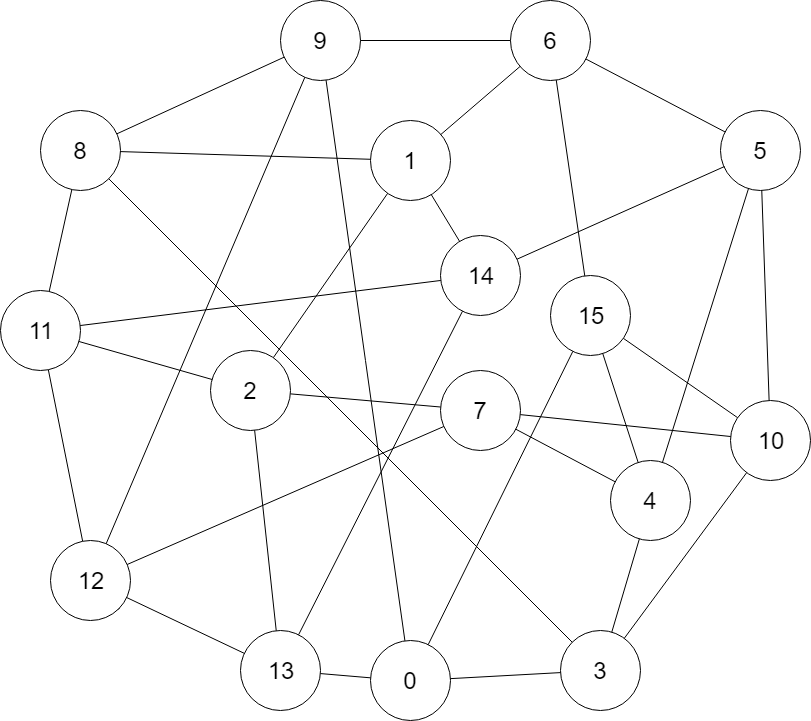
\includegraphics[width=.25\textwidth]{Network.png}
	\caption{Topological NW Model}
	\label{fig:topo}
	\end{center}
\end{figure}

\vspace{-8mm}
\begin{figure}[htb]
	\begin{center}
	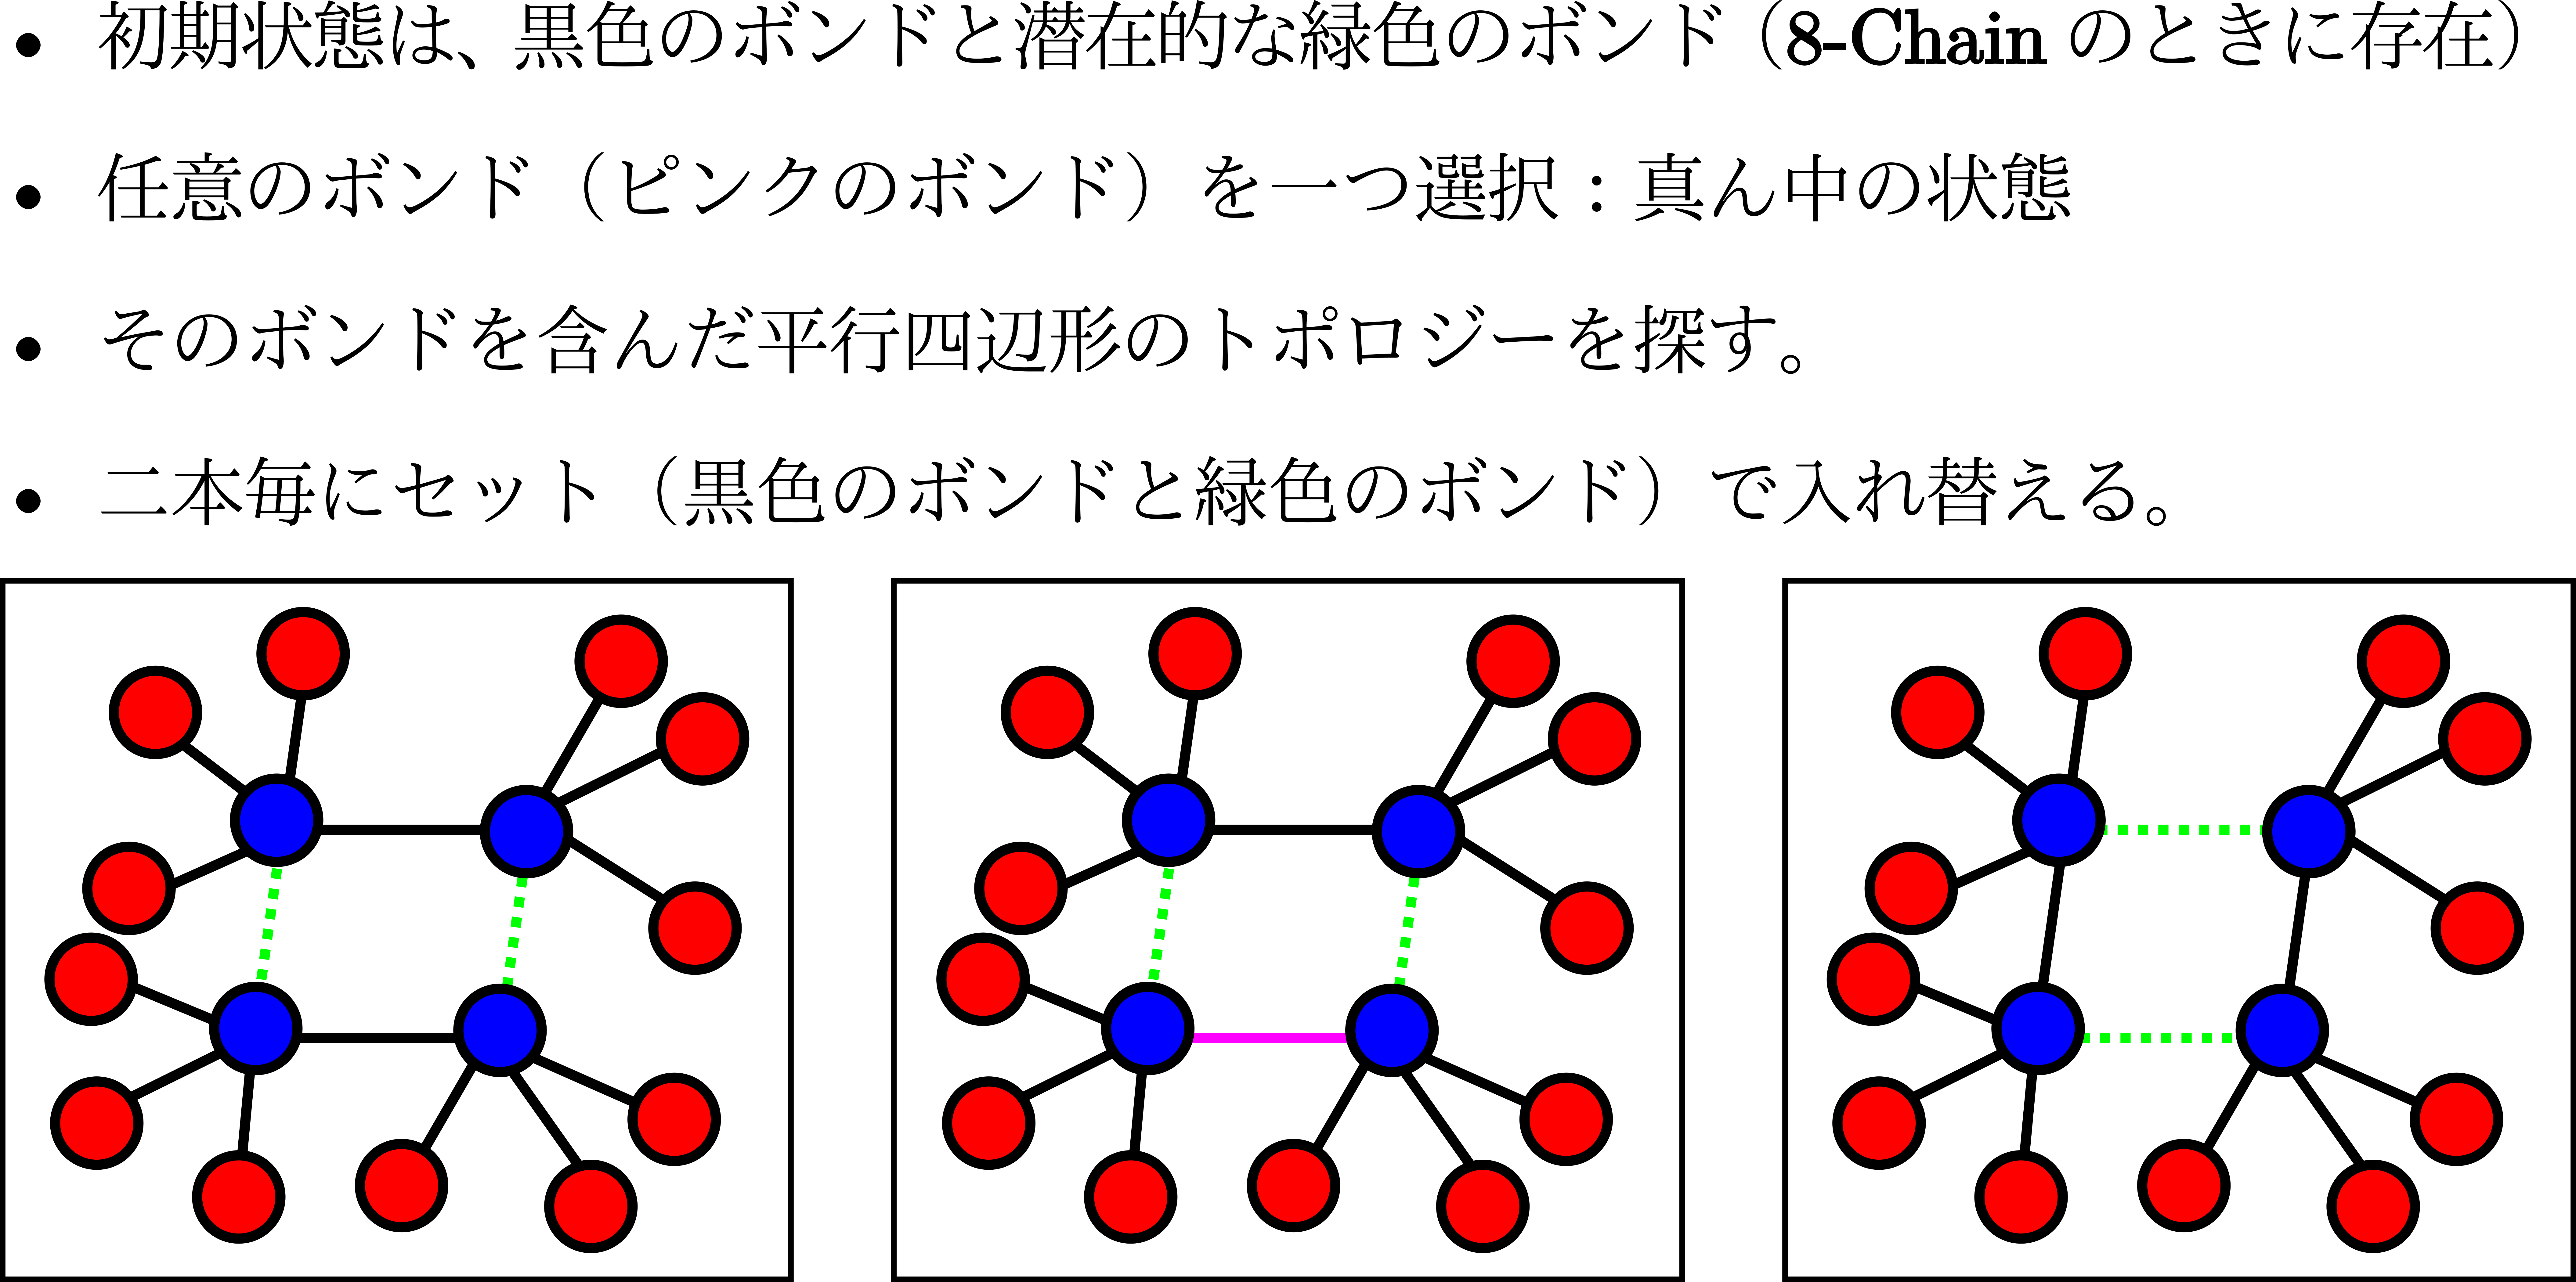
\includegraphics[width=.48\textwidth]{bond_exchg.png}
	\caption{Strand Exchange Procedure}
	\label{fig:exc}
	\end{center}
\end{figure}
\vspace{-5mm}

\subsection{ポテンシャルの設定}
非結合ポテンシャルは、斥力($r_c = 2^{(1/6)}\sigma$)である LJ ポテンシャル $U_{LJ}(r_{ij})$、ボンドポテンシャルには FENE-LJ ポテンシャルを用いて KG 鎖とした。
なお、初期構造の緩和は、Auhl 等の方法~\cite{Auhl2003a} に従い、force-capped-LJ ポテンシャルにより過剰な絡み合いを除外した。

% \vspace{-5mm}
\begin{figure}[htb]
	\centering
	   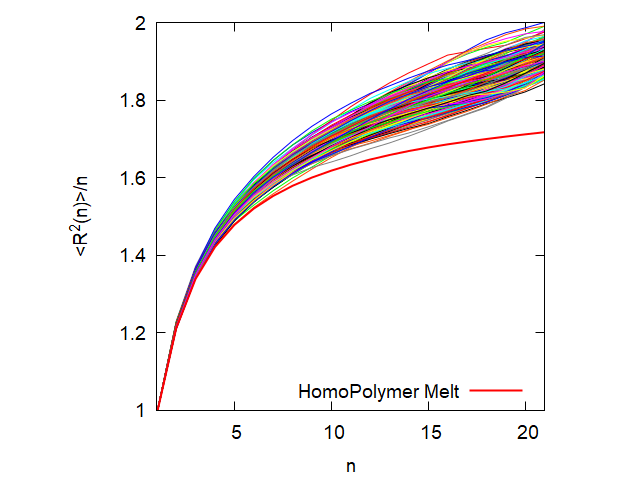
\includegraphics[width=.42\textwidth]{N20_f3_CN.png}
	%    \vspace{-5mm}
	   \caption{Mean Square Internal Distance distribution of strands}
	   \label{fig:e2e}
   \end{figure}
   \vspace{-5mm}
   
\section{結果と考察}
\vspace{-2mm}

ここでは、セグメント数 N=20 のストランドの三分岐モデルについてまとめた。

\subsection{ストランドのセグメント間距離 $\langle \bm{R} \rangle$ の分布関数}

ストランドの長手方向に沿ったセグメント間距離($n=21$ で末端間距離に対応)の分布関数の平衡状態でのトラジェクトリーを、ホモポリマーの平均値とともに Fig.\ref{fig:e2e} に示した。
セグメント数 5 程度までの部分鎖としての振る舞いは、拘束のないメルトポリマー鎖と同程度であった。
しかし、長い領域では伸びており、そのゆらぎは若干低下していた。
これは周期境界条件により、架橋点すなわちストランド末端が拘束された影響と考えられた。

\subsection{$\lambda =2$ からの応力緩和}
$\lambda =2$ まで迅速に伸長した後の応力緩和関数 $G(t)$ を Fig.\ref{fig:stress_rel} に示した。
緩和後の弾性率 $G_{eq} = 3.4E^{-2}$は、ANM よりも低下していたが PNM よりは大きいものであった。
この結果は、ネットワークにランダムな結合性は導入されファントム性が生じてはいるが、周期境界条件による拘束により効果が限定されたと推定できた。

\begin{figure}[htb]
 \centering
	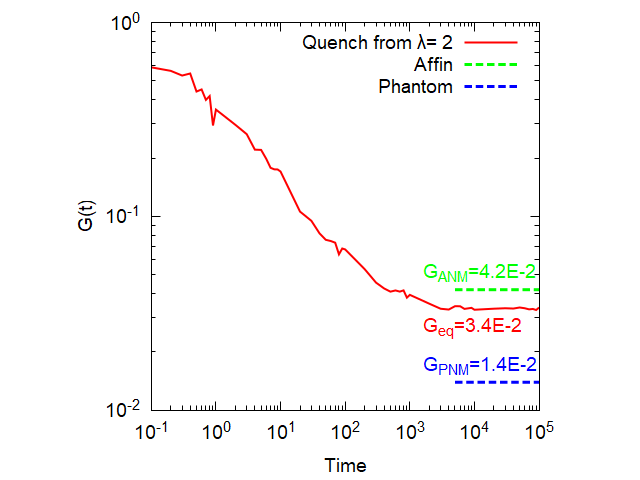
\includegraphics[width=.42\textwidth]{N20_f3_gt.png}
	% \vspace{-5mm}
	\caption{Stress Relaxation Curves for Uni-axial Step Strain($\lambda=2$)}
	\label{fig:stress_rel}
\end{figure}
\vspace{-5mm}

\bibliographystyle{../achemso}
%{elsart-num}
%{junsrt-2}
\bibliography{D:/Dropbox/Tex/Bibliography/library.bib}


\end{document}